\chapter{商取引ゲーム}
本章では、外部の強制執行力によって商取引契約の履行が保証されない商取引を「商取引ゲーム」としてモデリングし、
合理的な集団を仮定した場合に、そのゲームにおいて不正が生じないようなインセンティブを設計が不可能なことを示す。

% 社会契約が商取引の連鎖と捉えられることを示す
% \section{商取引の連鎖}
% 商取引とは、買い手と売り手の2者間で行われる通貨と商品(財もしくはサービスの提供)の交換である。
% この定義に従うと、この社会の複数人で行われる通貨や商品のやり取りは、全て商取引に分解することができる。
% 例えば1章の初めに述べたコーヒーの購入はもちろん、あなたとあなたと店主との間で行われるコーヒーと通貨の交換であるし、
% 警察が不正を取り締まるのも、あなたと警察官と政府の3者間で行われる商取引である。
% より詳細に考えるならば、あなたと政府との間で行われる通貨と公共サービスの交換と、
% 政府と警察官との間で行われる給料としての通貨と警察官業務というサービスの交換、2つの商取引である。
% 仮にイギリス人の金とインド人の胡椒の物々交換であったとしても、両者の通貨に価値を換算することで、
% 金と通貨の交換と通貨と胡椒の交換の2つの商取引といったように。
% それゆえ、1章1節で述べたような信頼の連鎖も複数の商取引に分解することができ、
% 本当に商取引契約が履行される強制力が存在しているならば、
% そのその連鎖の根源には必ず、他の商取引によって保証されることなく必ず履行される商取引が存在しているはずである。


% コンヴェンション
% \section{コンヴェンションと囚人のジレンマ}
% デイビッドヒュームは社会契約をコンヴェンションという概念を用いて説明しようとした。
% これは社会契約が果たされるのは、商取引によって両者の自分の欲しい物が手に入るためだとした。


% 両者に利益があるから守られている?本当にそうだろうか?
% デイビッドヒュームのコンベンションと似た事例として、〇〇の研究を紹介する。
% すたぐハントゲームを紹介する。
% しかし、我々は2者の戦略の結果が両者にとって最善になるからといって、
% 必ずしもそこに行きつけるわけではないことを囚人のジレンマから学んでいる。


% 問題提起
\section{本章の問題提起}
外部の強制執行力が存在すると仮定した上で、
合理的な人々が商取引を成功させるようなインセンティブ設計ができるか?

仮にそれをなし得る外部の強制力が存在していたとして、
1章の初めに述べたように、その存在というのは堂々巡りになっていく。
警察も、裁判所も、税金を支払うことによって受けているサービスという点で、
商取引だと考えれば、この商取引の依存関係を紐解いたさきに、
必ず1つは他の商取引に依存せずとも、契約が履行される商取引が存在しているはずである。
果たしてそんな商取引のメカニズムはデザイン可能なのか?

\section{本章の仮説}

\section{提案手法}

% 全員が行動は観察することができない
\section{行動観察不可の条件}

% アプローチ:無法地帯での商取引を考え、
\section{無法地帯での商取引}
この問いに答えるために、本章では無法地帯での商取引について考える。
商品(財・サービス)の引き渡しと通貨の支払いについて考える。
売り手と買い手(buyer)の2者間で行われる商取引。
外部の強制執行力は働かない。

商取引が成功したのか失敗したのかの報告を受けて、それに応じて各プレイヤーの通貨の保有量を変更するシステムである。

\subsection{商取引システム}
% TODO: 商取引システムについての概要をまとめる


% \section{第3者に依存しない仲介システム}
  商取引において不正行為を防止するためには,
  第3者に依存せずに動作の正当性が保証された商取引を仲介するシステムが存在していて,
  かつ,そのシステムは商取引で不正行為を防止できるインセンティブ設計を行える必要がある.
  仮に第3者に依存せずに動作の正当性が保証された仲介するシステムが存在しないとすれば,
  再帰的に,商取引を仲介するシステムの動作の正当性を保証する他の仲介するシステムが必要となるため,
  一向にそのシステムの正当性は保証されない.
  それ故,必ず第3者に依存せずに動作の正当性が保証された仲介するシステムが存在している必要がある.
  
  その上で,商取引において不正行為を防止するには,
  そのシステムから商取引の当事者達が不正行為を行わなくなるようなインセンティブ設計を行う必要がある.
  つまりは,第3者に依存せずに動作の正当性が保証されたシステム
  (本稿では,これを「第3者に依存しない仲介システム」と呼ぶ.)が存在しており,
  この「第3者に依存しない仲介システム」から商取引の不正行為防止のためのインセンティブ設計が行えなければならない.


% \section{行動観察不可の条件}
   仮にこのようなシステムが存在していたとして,このシステムからインセンティブ設計を行う際には,
  商取引の当事者である$seller$と$buyer$の行動を観察することができないという条件(以後,「行動観察不可の条件」と呼ぶ.)をおくべきである.
  なぜなら,商取引が失敗した場合に$seller$と$buyer$のどちらに非があるかを確かめるには,
  第3者に依存せずに動作の正当性が保証されているという前提に反して,誰かしらの第3者に依存する必要があるからである.

  例えば,りんごの売買契約を結んだ$seller$と$buyer$がいて,
  どちらかがシステムにその商取引の失敗を報告したとする.
  ここで$seller$と$buyer$のどちらが不正行為を行ったかを知るために,
  代理人を選出して調査を行うことや,
  りんごにシステムから不正行為を検知するためのセンサーをあらかじめ埋め込むなどの方法がある.
  しかし,どちらも代理人やセンサーの正当性を保証する製造者などの第3者に依存してしまう.
  また,代理人や製造者が正当性が保証されたシステムの一部であると仮定しても,
  第3者である彼らの正当性が保証されているためには,
  別の「第3者に依存しない仲介システム」を用いて彼らと商取引を結んでいなければならず,
  その仮定は別の「第3者に依存しない仲介システム」という第3者に依存していることを前提としてしまう.

  つまり,商取引において不正行為を防止するためには,「行動観察不可の条件」を満たす「第3者に依存しない仲介システム」が存在していなければならないのである.

% \section{商取引システム}
 この「行動観察不可の条件」を満たす「第3者に依存しない仲介システム」が存在するのかを論じるために,このシステムに以下の条件を付随したものを「商取引システム」と定義する.
  \begin{itemize}
    \item このシステム内には通貨が存在している.
    \item このシステムからは各$player$(システムの参加者)の通貨の保有量を観察・操作することができる.
    \item このシステムを仲介として商取引を行う際,支払いはシステム内の通貨で行われる.
    \item このシステムは商取引の当事者(本稿では$buyer$)から結果の報告を受けた際に各$player$の通貨の保有量を任意に操作する.
  \end{itemize}
\section{商取引ゲーム}
 また,この「商取引システム」において,商取引で不正行為を防止できるインセンティブ設計を行うことができるのかを検証するするために,
  このシステムを商取引の仲介として用いる「商取引ゲーム」を次のように定義する.なお,ここでのゲームの$players$(システムの参加者達)は合理的に(期待利得の最も高い)戦略を決定するものとする.
  
  \subsection{ゲームの進め方}
   本稿での商取引は,以下の4つのステップで$seller$と$buyer$が交互に行動を展開するものとする.
  
    \begin{description}
      \item[step1] $seller$は商品$goods$とその価格を告知する
      \item[step2]  その商品の購入を希望する$buyer$が「商取引システム」に商取引の合意を報告する.
      \item[step3]  $seller$は「正当な行為」と「不正な行為」のどちらかの行動選択をする.ここで「正当な行為」を行った場合,$buyer$は契約通りの$goods$を受け取れ, 「不正な行為」を行った場合,$buyer$は契約通りの$goods$を受け取れないものとする.
      \item[step4]  $buyer$は商取引の「成功」か「失敗」かを「商取引システム」に報告する.この報告に基づき,「商取引システム」は$ seller$と$ buyer$の保有する通貨の量を調整する.
    \end{description}

  \subsection{ゲーム木}
    \begin{figure*}[h]
      \centering
      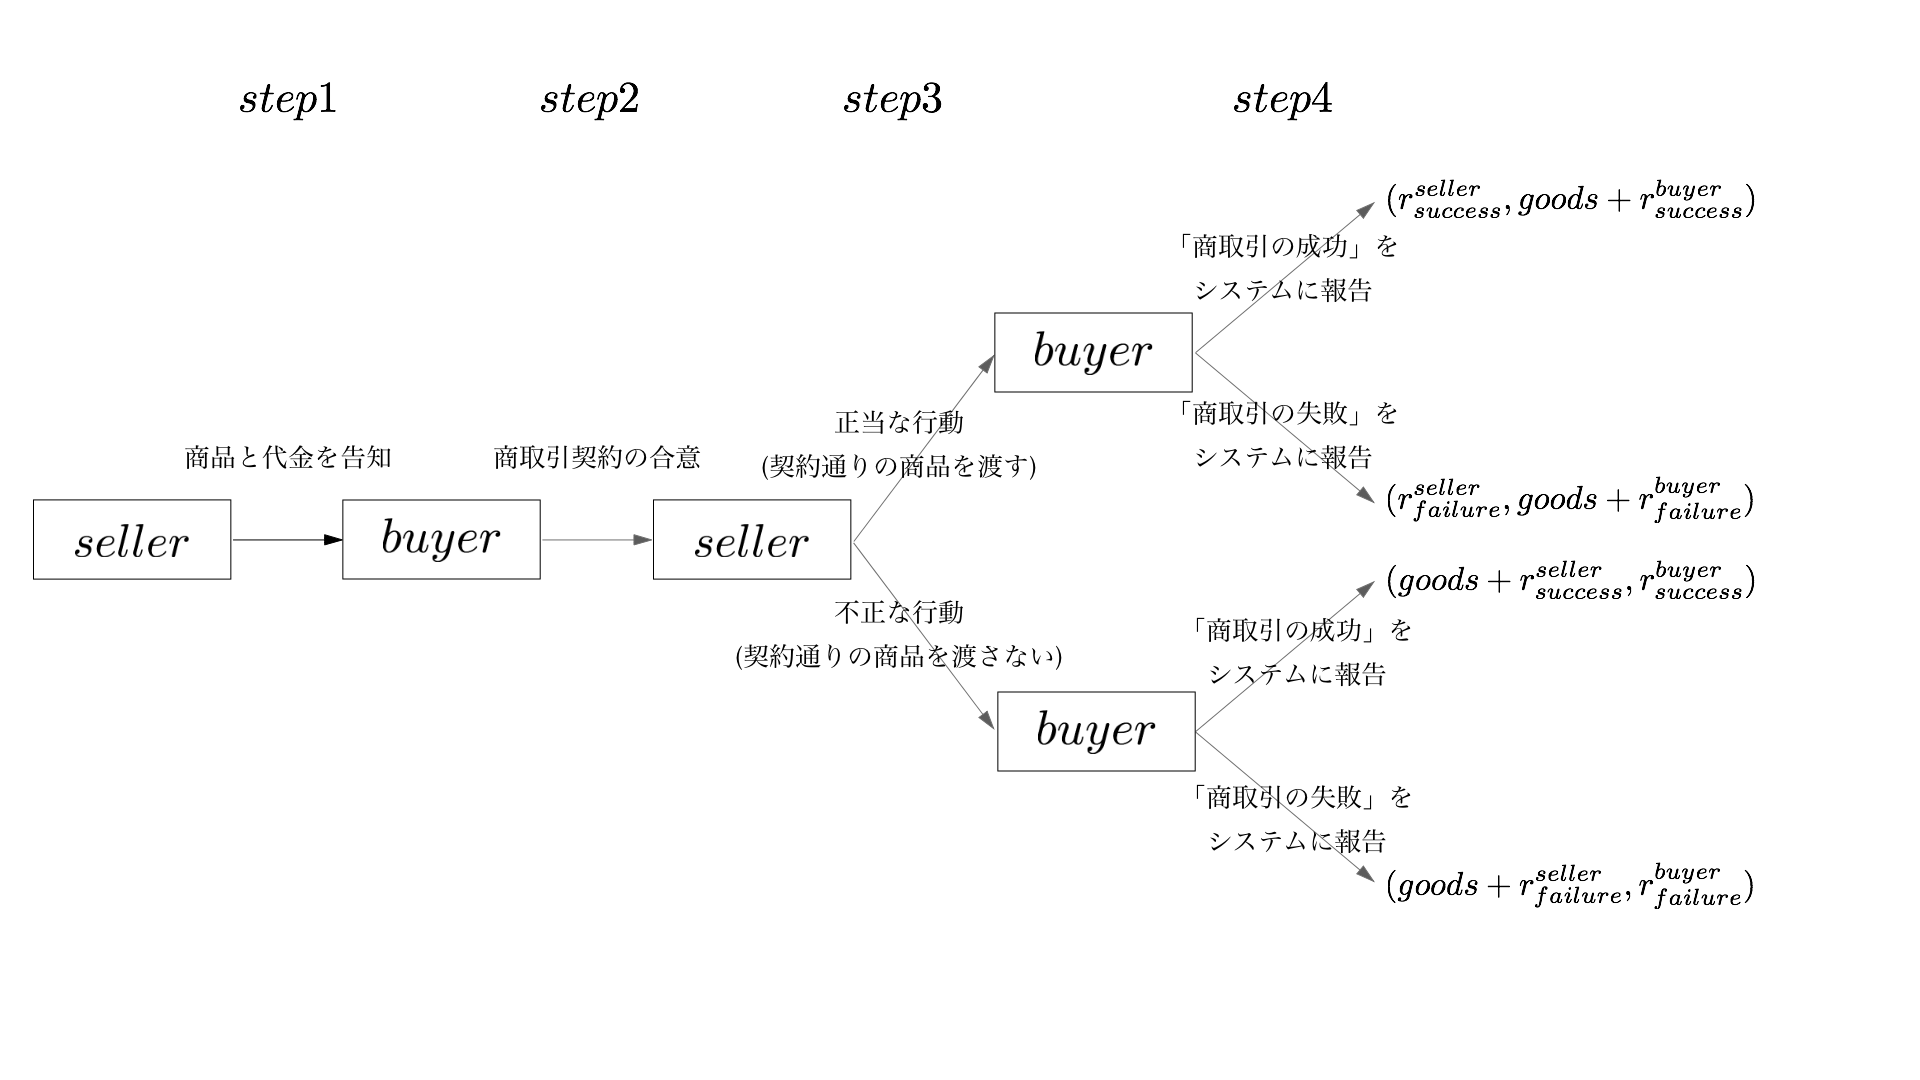
\includegraphics[width=1\linewidth]{./05_commerce-game/gametree.png}
      \caption{「商取引ゲーム」のゲーム木}
      \label{gametree}
    \end{figure*}
     先の商取引ゲームをゲームの木を用いて表すと図\ref{gametree}のようになる.\textbf{step1}と\textbf{step2}の時点では商取引の結果が変化することはなく,\textbf{step3}で$seller$が「正当な行為」をとるか否かと,\textbf{step4}での$buyer$からの報告によってのみ商取引の結果は変化する.また,「商取引システム」からは「行動観察不可の条件」より$seller$と$buyer$がどの行動をとったかはわからないため,\textbf{step4}での$buyer$の報告にのみ基づいて$seller$と$buyer$の保有する通貨の量を調整しなければならない.つまりは商取引の結果①と③,②と④はそれぞれ$goods$を除く利得は同じでなくてはならない.
  
  \subsection{非協力戦略型ゲーム}
    \newcommand{\successseller}{
      \begin{tabular}{c}
        $(r^{seller}_{success},$\\
        $goods+r^{buyer}_{success})$
      \end{tabular}
    }
    \newcommand{\successbuyer}{
      \begin{tabular}{c}
        $(goods+r^{seller}_{success},$\\
        $r^{buyer}_{success})$
      \end{tabular}
    }
    \newcommand{\fseller}{
      \begin{tabular}{c}
        $(r^{seller}_{failure},$\\
        $goods+r^{buyer}_{failure})$
      \end{tabular}
    }
    \newcommand{\fbuyer}{
      \begin{tabular}{c}
        $(goods+r^{seller}_{failure},$\\
        $r^{buyer}_{failure})$
      \end{tabular}
    }

    \begin{table*}[h]
      \begin{tabular}{|l|l|l|l|l|l|}
      \hline
      \multicolumn{2}{|l|}{\multirow{2}{*}{}} & \multicolumn{4}{l|}{$buyer$} \\ \cline{3-6}
      \multicolumn{2}{|l|}{}                  &$s^{buyer}_1$&$s^{buyer}_2$&$s^{buyer}_3$&$s^{buyer}_4$\\ \hline
      \multirow{2}{*}{$seller$}
      &$s^{seller}_1$&\successseller&\successseller&\fseller&\fseller\\ \cline{2-6}
      &$s^{seller}_2$&\fbuyer&\successbuyer&\fbuyer&\successbuyer\\ \hline
      \end{tabular}
      \caption{非協力戦略型ゲームとして表した「商取引ゲーム」の利得表}
      \label{gametable}
    \end{table*}
      
      また,この商取引のモデルは,第3ステップ以降の$seller$の行動選択と,それに対する第4ステップの$ buyer$の行動選択を,非協力戦略型ゲームとしてとらえられる.ここで,戦略$ s^{player}_{n}$を$ player$(ここでは$seller$か$buyer$)の取りうる戦略番号$n$の戦略として,$ seller$と$ buyer$のそれぞれの戦略は以下のように定義する.\\
      
      \begin{description}
        \item[$s^{seller}_1$]… 正当な行為を行う
        \item[$s^{seller}_2$]… 不正な行為を行う
        \item[$s^{buyer}_1$]… $ seller$が正当な行為をとった場合は「成功」を,不正な行動をとった場合は「失敗」を報告する
        \item[$s^{buyer}_2$]… $ seller$が正当な行為をとった場合は「成功」を,不正な行動をとった場合は「成功」を報告する
        \item[$s^{buyer}_3$]… $ seller$が正当な行為をとった場合は「失敗」を,不正な行動をとった場合は「失敗」を報告する
        \item[$s^{buyer}_4$]… $ seller$が正当な行為をとった場合は「失敗」を,不正な行動をとった場合は「成功」を報告する
      \end{description}
      
      また,商取引終了時の$ player$の保有する通貨量の変化によって生じる利得を,第4ステップでの報告が「成功」だった場合は$ r^{player}_{success}$,「失敗」だった場合は$ r^{player}_{failure}$とし,商品の所有によって生じる利得を$ goods$と表す.
      ここで,$ seller$と$ buyer$の任意の戦略組$ (s^{seller}_n, s^{buyer}_n)$の際の$ seller$と$ buyer$の各利得は表\ref{gametable}のようになる.
      
\section{不可能性の証明}
\subsection{前提の整理}
  \begin{itemize}
    \item システムは$buyer$によって報告された商取引の結果を観察できる.
    % \vspace{-12mm}
    \item システムは$seller$と$buyer$がどの戦略を選んだかはわからない.
    % \vspace{-12mm}
    \item 商取引に参加する$player$は合理的に(利得の期待値が最も高い)戦略を決定する.
    % \vspace{-12mm}
    \item システム内には追跡可能な通貨が存在しており,商取引にはその通貨が用いられる.
    % \vspace{-12mm}
    \item システムからは$player$の通貨の保有量を操作することができる.
    % \vspace{-12mm}
  \end{itemize}

\subsection{不正行為が起きない戦略組とその条件}
 表より,商取引で不正行為が起きないためには,$seller$と$buyer$のとる戦略組が$ (s^{seller}_1, s^{buyer}_1)$もしくは$(s^{seller}_1, s^{buyer}_2)$のいずれかに帰着しなければならない.

  ここで$player$が戦略$s^{player}_n$をとったときの利得$R$の期待値を$E(R|s^{player}_n)$とする.

  $(s^{seller}_1, s^{buyer}_1)$に帰着するためには,\\

  $E(R|s^{seller}_1)>E(R|s^{seller}_2)$
  かつ
  $E(R|s^{buyer}_1)>E(R|s^{buyer}_2)$
  かつ
  $E(R|s^{buyer}_1)>E(R|s^{buyer}_3)$
  かつ
  $E(R|s^{buyer}_1)>E(R|s^{buyer}_4)$ …条件①\\

  を満たす必要があり,$(s^{seller}_1, s^{buyer}_2)$に帰着する場合は,\\

  $E(R|s^{seller}_1)>E(R|s^{seller}_2)$
  かつ
  $E(R|s^{buyer}_2)>E(R|s^{buyer}_1)$
  かつ
  $E(R|s^{buyer}_2) > E(R|s^{buyer}_3)$
  かつ
  $E(R|s^{buyer}_2) > E(R|s^{buyer}_4)$ …条件②\\

  を満たす必要がある.\\

   つまり,不正行為を防ぐ商取引のインセンティブ設計を行うためには,条件①もしくは条件②を満たす$(r^{seller}_{success}, r^{seller}_{failure}, r^{buyer}_{success}, r^{buyer}_{failure})$の組を「商取引システム」から決定することができなければならない.
  そこで,不正行為を防ぐ商取引のインセンティブ設計が不可能であることを示すために,次の命題を証明する.

\subsection{命題}
条件①もしくは条件②のいづれかの条件を満たす$(r^{seller}_{success}, r^{seller}_{failure}, r^{buyer}_{success}, r^{buyer}_{failure})$の組を商取引システムから決定することはできない.

\subsection{証明}
$player$が戦略$s^{player}_n$をとる確率を$p^{player}_{n}$と表す.$(0 \leq p^{player}_{n} \leq 1)$\\

$seller$について,各戦略の期待利得は以下のように表せる. \\
$E(R|s^{seller}_1)=p^{buyer}_1{r}^{seller}_{success}+p^{buyer}_2r^{seller}_{suceess}+p^{buyer}_3r^{seller}_{failure}+p^{buyer}_4r^{seller}_{failure}$ \\

$ E(R |s^{seller}_2) = p^{buyer}_1 (goods + r^{seller}_{failure}) + p^{buyer}_2 (goods + r^{seller}_{success}) + p^{buyer}_3 (goods + r^{seller}_{failure} ) + p^{buyer}_4 (goods + r^{seller}_{success})$ \\

$ = goods + p^{buyer}_1 r^{seller}_{failure} + p^{buyer}_2 r^{seller}_{success} + p^{buyer}_3 r^{seller}_{failure} + p^{buyer}_4 r^{seller}_{success}$ \\

ここで,$E(R |s^{seller}_1) > E(R |s^{seller}_2)$ を満たすためには, \\
$p^{buyer}_1 {r}^{seller}_{success} + p^{buyer}_2 r^{seller}_{suceess} + p^{buyer}_3 r^{seller}_{failure} + p^{buyer}_4 r^{seller}_{failure}$ \\

$ > goods + p^{buyer}_1 r^{seller}_{failure} + p^{buyer}_2 r^{seller}_{success} + p^{buyer}_3 r^{seller}_{failure} + p^{buyer}_4 r^{seller}_{success}$ \\

 $\therefore p^{buyer}_1 {r}^{seller}_{success} +  p^{buyer}_4 r^{seller}_{failure} > goods + p^{buyer}_1 r^{seller}_{failure} + p^{buyer}_4 r^{seller}_{success}$ \\

$\therefore p^{buyer}_1 {r}^{seller}_{success} +  p^{buyer}_4 r^{seller}_{failure} - goods + p^{buyer}_1 r^{seller}_{failure} - p^{buyer}_4 r^{seller}_{success} > 0$ \\

$\therefore p^{buyer}_1(r^{seller}_{success} - r^{seller}_{failure}) - p^{buyer}_4(r^{seller}_{success} - r^{seller}_{failure} ) - goods > 0$ \\

$\therefore (p^{buyer}_1 - p^{buyer}_4)(r^{seller}_{success} - r^{seller}_{failure}) - goods> 0$ \\

$\therefore (p^{buyer}_1 - p^{buyer}_4)(r^{seller}_{success} - r^{seller}_{failure} - \frac{ goods }{p^{buyer}_1 - p^{buyer}_4})> 0$ \\
を満たす必要がある.つまり,\\

$ p^{buyer}_1>p^{buyer}_4$のときは, \\

$ r^{seller}_{success} - r^{seller}_{failure} > \frac{ goods }{p^{buyer}_1 - p^{buyer}_4}$\\

$ p^{buyer}_1 < p^{buyer}_4$のときは,\\

$ r^{seller}_{success} - r^{seller}_{failure} < \frac{ goods }{p^{buyer}_1 - p^{buyer}_4}$\\

を満たせば,$E(R |s^{seller}_1) > E(R |s^{seller}_2)$である.
なお,$ p^{buyer}_1 = p^{buyer}_4$のときは,\\

$E(R |s^{seller}_1) > E(R |s^{seller}_2)$は成り立たない.\\

また,$ {buyer}$について,各戦略の期待利得は以下のように表せる.\\

$ E(R|s^{buyer}_1) = p^{seller}_1 (goods + r^{buyer}_{success}) + p^{seller}_2 r^{buyer}_{failure}$ \\

$ E(R|s^{buyer}_2)=p^{seller}_1 (goods + r^{buyer}_{success}) + p^{seller}_2 r^{buyer}_{success}$ \\

$ E(R|s^{buyer}_3)=p^{seller}_1 (goods + r^{buyer}_{failure}) + p^{seller}_2 r^{buyer}_{failure}$ \\

$ E(R|s^{buyer}_4)=p^{seller}_1 (goods + r^{buyer}_{failure}) + p^{seller}_2 r^{buyer}_{success}$ \\

\subsubsection{条件①が成り立たないことの証明}

ここで,条件①の必要条件である
$E(R|s^{buyer}_1)>E(R|s^{buyer}_2)$
かつ
$E(R|s^{buyer}_1)>E(R|s^{buyer}_3)$
かつ
$E(R|s^{buyer}_1)>E(R|s^{buyer}_4)$
を満たすためには,\\

$ E(R|s^{buyer}_1) > E(R|s^{buyer}_2)$ \\

$\therefore p^{seller}_1 (goods + r^{buyer}_{success}) + p^{seller}_2 r^{buyer}_{failure} > p^{seller}_1 (goods + r^{buyer}_{success}) + p^{seller}_2 r^{buyer}_{success}$ \\

$\therefore p^{seller}_2 r^{buyer}_{failure} - p^{seller}_2 r^{buyer}_{success} > 0$ \\

$\therefore p^{seller}_2 (r^{buyer}_{failure} - r^{buyer}_{success}) > 0$ \\

つまり,$ p^{seller}_2 > 0$ かつ $ r^{buyer}_{failure} - r^{buyer}_{success} > 0$

\begin{equation}
  p^{seller}_2 > 0
\end{equation}

\begin{equation}
\label{quad1}
  0 > r^{buyer}_{success} - r^{buyer}_{failure}
\end{equation}

$ E(R|s^{buyer}_1) > E(R|s^{buyer}_3)$ \\

$ \therefore p^{seller}_1(goods + r^{buyer}_{success}) + p^{seller}_2r^{buyer}_{failure}>
  p^{seller}_1(goods + r^{buyer}_{failure}) + p^{seller}_2r^{buyer}_{failure}$\\

$ \therefore p^{seller}_1 (r^{bueyer}_{success} - r^{buyer}_{failure}) > 0$\\

つまり,$ p^{seller}_1 > 0$ かつ $r^{bueyer}_{success} - r^{buyer}_{failure} > 0$\\

\begin{equation}
   p^{seller}_1 > 0
\end{equation}
\begin{equation}
   \label{quad2}
   r^{buyer}_{success} - r^{buyer}_{failure} > 0
\end{equation}

$ E(R|s^{buyer}_1) > E(R|s^{buyer}_4)$ \\

$\therefore p^{seller}_1 (goods + r^{buyer}_{success}) + p^{seller}_2 r^{buyer}_{failure} > p^{seller}_1 (goods + r^{buyer}_{failure}) + p^{seller}_2 r^{buyer}_{success}$ \\

$\therefore p^{seller}_1(r^{buyer}_{success} - r^{buyer}_{failure}) + p^{seller}_2(r^{buyer}_{failure} - r^{buyer}_{success}) > 0$ \\

$ (p^{seller}_1 - p^{seller}_2)(r^{buyer}_{success} - r^{buyer}_{failure}) > 0$\\

\begin{equation}
\label{quad3}
  (p^{seller}_1 - p^{seller}_2)(r^{buyer}_{success} - r^{buyer}_{failure}) > 0
\end{equation}

の3つを満たす必要がある.しかし,(\ref{quad1})と(\ref{quad2})は矛盾するため,
$(r^{seller}_{success}, r^{seller}_{failure}, $
$r^{buyer}_{success}, r^{buyer}_{failure})$ \\
がいかなる実数の組でも条件①は成り立たない. \\


\subsubsection{条件②が成り立たないことの証明}
また,条件②の必要条件である
$E(R|s^{seller}_1)>E(R|s^{seller}_2)$
かつ
$E(R|s^{buyer}_2)>E(R|s^{buyer}_1)$
かつ
$E(R|s^{buyer}_2) > E(R|s^{buyer}_3)$
かつ
$E(R|s^{buyer}_2) > E(R|s^{buyer}_4)$
を満たすためには,

$ E(R|s^{buyer}_2) > E(R|s^{buyer}_1)$ \\

$\therefore p^{seller}_1 (goods + r^{buyer}_{success}) + p^{seller}_2 r^{buyer}_{success} > p^{seller}_1 (goods + r^{buyer}_{success}) + p^{seller}_2 r^{buyer}_{failure}$\\

$\therefore p^{seller}_2 (r^{buyer}_{success} - r^{buyer}_{failure}) > 0$\\

$0 \leq p^{seller}_2 \leq 1$より,\\

$p^{seller}_2 > 0$かつ
$r^{buyer}_{success} - r^{buyer}_{failure} > 0$\\

\begin{equation}
  p^{seller}_2 > 0
\end{equation}

\begin{equation}
  \label{quad2-1}
  r^{buyer}_{success} - r^{buyer}_{failure} > 0
\end{equation}

$ E(R|s^{buyer}_2) > E(R|s^{buyer}_3)$\\

$\therefore p^{seller}_1 (goods + r^{buyer}_{success}) + p^{seller}_2 r^{buyer}_{success} > p^{seller}_1 (goods + r^{buyer}_{failure}) + p^{seller}_2 r^{buyer}_{failure}$\\

$\therefore p^{seller}_1 (r^{buyer}_{success} - r^{buyer}_{failure}) + p^{seller}_2 (r^{buyer}_{success} - r^{buyer}_{failure}) > 0$\\

$\therefore (p^{seller}_1 + p^{seller}_2)(r^{buyer}_{success} - r^{buyer}_{failure}) > 0$\\

$ p^{seller}_1 + p^{seller}_2 = 1 > 0$より,\\

$ r^{buyer}_{success} - r^{buyer}_{failure} > 0$\\

\begin{equation}
  \label{quad2-2}
  r^{buyer}_{success} - r^{buyer}_{failure} > 0
\end{equation}

$ E(R|s^{buyer}_2) > E(R|s^{buyer}_4)$\\

$\therefore p^{seller}_1 (goods + r^{buyer}_{success}) + p^{seller}_2 r^{buyer}_{success} > p^{seller}_1 (goods + r^{buyer}_{failure}) + p^{seller}_2 r^{buyer}_{success}$\\

$\therefore p^{seller}_1(r^{buyer}_{success} - r^{buyer}_{failure}) > 0$\\

$ p^{seller}_1 > 0$かつ
$ r^{buyer}_{success} - r^{buyer}_{failure} > 0$\\

\begin{equation}
  p^{seller}_1 > 0
\end{equation}

\begin{equation}
  \label{quad2-3}
  r^{buyer}_{success} - r^{buyer}_{failure} > 0
\end{equation}

ここで,(\ref{quad2-1}),(\ref{quad2-2}),(\ref{quad2-3})を満たす
$ (r^{buyer}_{success}, r^{buyer}_{failure})$の組はシステムから決定できるため,\\

$p^{seller}_2>0$かつ$p^{seller}_1>0$であれば,

$E(R|s^{buyer}_2)>E(R|s^{buyer}_1)$
かつ
$E(R|s^{buyer}_2) > E(R|s^{buyer}_3)$
かつ
$E(R|s^{buyer}_2) > E(R|s^{buyer}_4)$
を満たすことができる.\\

ここで仮に$p^{seller}_2>0$かつ$p^{seller}_1>0$が成り立ち$ buyer$が戦略$ s^{buyer}_2$を選択するととする.\\

このとき,$buyer$が各戦略をとる確率$(p^{buyer}_1, p^{buyer}_2, p^{buyer}_3, p^{buyer}_4)$は$ (0, 1, 0, 0)$と表せる.\\

ここで,$ p^{buyer}_1 = p^{buyer}_4 = 0$のため,
$E(R |s^{seller}_1) > E(R |s^{seller}_2)$は成り立たない.\\

それゆえに,条件②は成り立たない.\\

以上より,条件①もしくは条件②のいづれかの条件を満たす
$(r^{seller}_{success}, r^{seller}_{failure},$
$r^{buyer}_{success},r^{buyer}_{failure})$の組を「商取引システム」から決定することはできない.\\


\section{結論}
   本稿では,商取引において不正行為を防止するためには,「行動観察不可の条件」を満たした「第3者に依存しない仲介システム」が存在している必要があることを論じた.その上で,そのシステムが存在するのかを検証するために,下記の条件を付随した「商取引システム」と,それを仲介とした「商取引ゲーム」を定義して,商取引で不正行為を防止できるインセンティブ設計が可能かを確かめた.

  \begin{itemize}
    \item システムは$buyer$によって報告された商取引の結果を観察できる.
    \item システムは$seller$と$buyer$がどの戦略を選んだかはわからない.
    \item 商取引に参加する$player$は合理的に(利得の期待値が最も高い)戦略を決定する.
    \item システム内には追跡可能な通貨が存在しており,商取引にはその通貨が用いられる.
    \item システムからは$player$の通貨の保有量を操作することができる.
  \end{itemize}

  その結果として,不正行為が防止されるための2つの戦略組のいずれかに$seller$と$buyer$の戦略を帰着させるような利得の組を商取引システムから決定することはできないことを証明した.これはつまり,人々は合理的であるという仮定の上で成り立つ「商取引ゲーム」において,不正行為を防止することが不可能であることを意味する.


社会契約は複数の商取引の連鎖と捉えることができる。
デイビッドヒュームは同じように考えて、商取引において双方にメリットがあるから社会契約は成立すると考えた。
囚人のジレンマから必ずしもパレート最適な答えにたどり着くわけではないことがわかる。
商取引において、不正を防止するインセンティブ設計は可能か?
無法地帯での無人売買機問題
商取引システム